\documentclass[12pt]{scrartcl}
\usepackage[sexy]{james}
\usepackage[noend]{algpseudocode}
\setlength{\marginparwidth}{2cm}
\usepackage{answers}
\usepackage{array}
\usepackage{tikz}
\newenvironment{allintypewriter}{\ttfamily}{\par}
\usepackage{listings}
\usepackage{xcolor}
\usetikzlibrary{arrows.meta}
\usepackage{color}
\usepackage{mathtools}
\usepackage{graphicx}
\newcommand{\U}{\mathcal{U}}
\newcommand{\E}{\mathbb{E}}
\newcommand{\V}{\text{Var}}
\newcommand{\C}{\text{Cov}}
\usetikzlibrary{arrows}
\Newassociation{hint}{hintitem}{all-hints}
\renewcommand{\solutionextension}{out}
\renewenvironment{hintitem}[1]{\item[\bfseries #1.]}{}
\renewcommand{\O}{\mathcal{O}}
\declaretheorem[style=thmbluebox,name={Chinese Remainder Theorem}]{CRT}
\renewcommand{\theCRT}{\Alph{CRT}}
\setlength\parindent{0pt}
\usepackage{sansmath}
\usepackage{pgfplots}

\usetikzlibrary{automata}
\usetikzlibrary{positioning}  %                 ...positioning nodes
\usetikzlibrary{arrows}       %                 ...customizing arrows
\newcommand{\eqdef}{=\vcentcolon}
\newcommand{\tr}{{\rm tr\ }}
\newcommand{\im}{{\rm Im\ }}
\newcommand{\spann}{{\rm span\ }}
\newcommand{\Col}{{\rm Col\ }}
\newcommand{\Row}{{\rm Row\ }}
\newcommand{\dint}{\displaystyle\int}
\newcommand{\dt}{\ {\rm d }t}
\newcommand{\PP}{\mathbb{P}}
\newcommand{\Var}{\text{Var}}
\newcommand{\horizontal}{\par\noindent\rule{\textwidth}{0.4pt}}
\usepackage[top=3cm,left=3cm,right=3cm,bottom=3cm]{geometry}
\newcommand{\mref}[3][red]{\hypersetup{linkcolor=#1}\cref{#2}{#3}\hypersetup{linkcolor=blue}}%<<<changed

\tikzset{node distance=4.5cm, % Minimum distance between two nodes. Change if necessary.
         every state/.style={ % Sets the properties for each state
           semithick,
           fill=cyan!40},
         initial text={},     % No label on start arrow
         double distance=4pt, % Adjust appearance of accept states
         every edge/.style={  % Sets the properties for each transition
         draw,
           ->,>=stealth',     % Makes edges directed with bold arrowheads
           auto,
           semithick}}


% Start of document.
\newcommand{\sep}{\hspace*{.5em}}

\pgfplotsset{compat=1.18}
\begin{document}
\title{BUFN402: Portfolio Management}
\author{James Zhang\thanks{Email: \mailto{jzhang72@terpmail.umd.edu}}}
\date{\today}

\definecolor{dkgreen}{rgb}{0,0.6,0}
\definecolor{gray}{rgb}{0.5,0.5,0.5}
\definecolor{mauve}{rgb}{0.58,0,0.82}

\lstset{frame=tb,
  language=Java,
  aboveskip=3mm,
  belowskip=3mm,
  showstringspaces=false,
  columns=flexible,
  basicstyle={\small\ttfamily},
  numbers=left,
  numberstyle=\tiny\color{gray},
  keywordstyle=\color{blue},
  commentstyle=\color{dkgreen},
  stringstyle=\color{mauve},
  breaklines=true,
  breakatwhitespace=true,
  tabsize=3
}

\maketitle
    These are my (``live-\TeX``-ed) notes for UMD's BUFN402: Portfolio Management, 
    which is a required class in the Computational Finance Minor. This course is taught by Professor Seokwoo Lee. 
\tableofcontents
\newpage

\section{Intro}

Hey guys, let's learn the skills needed to becomne junior quant researchers!

\section{Probability Theory}

See Professor Lee's comprehensive slideshow on the probability theory concepts that 
we need to know.


\section{Simple PF Theory}

\begin{example}
  \vocab{No Arbitrage Principle}. Consider a \vocab{default-free zero-coupon bond}
  paying you $\$1000$ in one year. Assume risk-free interest rate is 
  $\$5$ and the financial market is well functioning and competitive. Suppose 
  the bond is traded for $\$940$. Is there an arbitrage opportunity? 

  \begin{proof}[Solution]
    Buy the bond for $\$940$. At the same time, borrow $1.05x = 1000 \implies x = 952.38$
    from the bank. In 1 year, we get $1000$ from the bond which we give to the bank. Therefore, 
    we earn $12.38$ in cash today, without taking any risk or paying any of our money 
    in the future.
  \end{proof}

  What if the price of the bond is $960$. Is there an arbitrage opportunity?

  \begin{proof}[Solution]
    Sell the bond for $960$, then invest $952.38$ at the bank. In a year, it grows to 
    $1000$ and then you use it to pay off the bond. You keep $7.62$.
  \end{proof}
\end{example}

\begin{definition}
  In financial markets, it is possible to sell a security you do not own. This is called 
  \vocab{short-selling}. In short-selling, an investors borrows the security, sells it, and then 
  must either return the security by buying it back or pay the owner the cash flows 
  he would have received.
\end{definition}

\begin{note}
  The example above assumed no transaction costs and funding costs.
\end{note}

\includegraphics[width=14cm]{2_asset_frontier.png}

\begin{definition}
  The \vocab{efficient frontier} defines the best feasible set of PFs, given two 
  asset characteristics (mean and variance). Note that above, the red portions come 
  from allowing short selling. Also note the minimum variance PF. Additionally, note that 
  all PFs below the dotted red line are \vocab{inefficient} - that is, for the same 
  level of risk, you can obtain a PF with greater expected return.
\end{definition}

\begin{definition}
  A \vocab{mean-variance utility maximizer} wants to solve 
  \[\max_{w_1} \E(R_p) - \frac{\gamma}{2}\V(R_p)\]
  where $\gamma$ is known as \vocab{risk-aversion} and sometimes 
  $\tau = \frac{1}{\gamma}$ is \vocab{risk-tolerance}.
\end{definition}

\subsection{Frontiers with Risk-Free Assets}

\includegraphics[width=14cm]{frontier_utility.png}

\begin{remark}
  In addition to $2$ risky assets, suppose the investor can freely borrow and lend 
  at $r_f$. Consider a PF combining any PF on the frontier with the risk-free asset. 
  Then all feasible efficient PFs become on a line. 
\end{remark}

\begin{proof}[Solution]
  Let weight on a risky PF $R_p$ on the frontier be $w_p$ and so 
  $(1-w_p)$ to the risk-free asset. The return of the PF is then 
  \[R_{pf} = w_p R_p + (1-w_p)r_f\]
  \[\E(R_{pf}) = w_p\mu_p + (1-w_p)r_f\]
  \[\sigma(R_{pf})\ = w_p\sigma_p \implies (\sigma(R_{pf}, \E(R_{pf})))\]
  is linear in $w_p$ where the slope of this line is $\frac{(u_p - R_f)}{\sigma_p}$, \vocab{Sharpe Ratio}.
\end{proof}

\begin{note}
  The optimal PF for the mean variance utility maximizer becomes where their utility function 
  intersects with the line of maximum Sharpe Ratio.
\end{note}

\subsection{Long-Short Strategy of Hedge Fund}

Take notes on this later. Optional for now. 

\section{Capital Asset Pricing Model (CAPM)}

\begin{example}
  Let us construct an algorithm to find the efficient frontier with $N$ risky assets. 
  Vary target expected returns of the PF. Given $\mu_p$, minimize the 
  volatility of the PF by finding the weights subject to 
  \begin{itemize}
    \item $\sum w_i = 1$
    \item $\E(R_p) = \sum w_i \E(R_i)$
    \item $0 \leq w_i \ \forall \ i \in [1, N]$
  \end{itemize}
  Note that the last constraint is omitted if short selling is allowed. Additional 
  constraints can be added to customize the PF selection process. 

  More formally, the optimization step is states as follows. For a given target
  expected return $r_p$: 
  \[\min_{w} w^T \sigma w \text{ subject to } 1^T w = 1, w^T\mu = \mu_p, w \geq 0\]

  To find the \vocab{tangent PF}, which ist he PF with maximum Sharpe Ratio, 
  solve 
  \[\max_w \dfrac{\mu^t w - r_f}{\sqrt{w^T \sigma w}} \text{ subject to } 1^Tw = 1, w \geq 0\]

  The \vocab{global minimum variance PF} is easy to find in this methodology.
\end{example}

\begin{note}
  Suppose now that your investment universe is all tradeable assets. Then the 
  tangent PF is efficient and contains all assets. 
\end{note}

\begin{note}
  IMPORTANT: even if two investors have different risk tolerances, they still hold 
  the \vocab{same risky tangent PF $T$} just with different weight to the 
  tangent PF weights. Additionally, each weighting of the tangent PF 
  is directly correlated with the market. This is left as an exercise, it involves 
  computing the correlation coefficient between a weighted tangent PF and the market 
  and showing that it equals 1.
\end{note}

\subsection{CAPM Assumptions and Consequences}

\begin{note}
  Let us make four key assumptions for CAPM. 

  \begin{enumerate}[a.]
    \item Investors are mean-variance optimizers and take the market price as given.
    \item Two-periods - investors are planning to hold for one identical period 
    \item Investors all face the same investment opportunities, characterized by $N$ risky assets ,
    and they all borrow and lend at the same equilibrium risk free rate.
    \item \vocab{Rational Expectations} - all investors correctly interpret 
    any info they have and all information contained in asset prices, so all investors 
    will agree on expected returns, variances, and covariances of stocks.
  \end{enumerate}
\end{note}

\begin{note}
  Some important consequences of the above:
  \begin{enumerate}[a.]
    \item Each investor agrees on all assets' positions in $(\mu, \sigma)$ space. 
    \item Each investor identifies the same PF as having the highest Sharpe - same tangentPF 
    \item All investors demand the same tangent PF. Recall that different risk tolerances just adjust the weight of the 
    risk-free asset and the tangent PF 
    \item Because a security is owned by some, the sum of all investors' PFs must 
    equal the market PF. 
    \item If a security in the market were not part of the efficient {F}, then no investor would want it, and there is an excess supply of this asset. 
    This security's price would call, causing expected return to rise, until it became an attractive investment. In this way, prices in the market 
    will adjust so that the effiicent PF and the market PF coincide, and demand equals supply. This is essentially just a proof by contradiction.
    \item CAPM theory identifies the efficient PF as the market PF, and the market PF is easier to identify (SP500)
    \item Thus, if a mean-variance investor just performs regressions and not necessarily the mean-variance analysis themselves, 
    the investor can just use the market PF as the optimal tangent efficient PF.  
  \end{enumerate}
\end{note}

\subsection{CAPM Derivation}

\begin{proof}
  
  \[\vdots\]
  Therefore, the market PF is indeed mean-variance efficient. Hence 
  \[\E(R_i) - r_f = \beta_{i, m} (\E(R_m) - r_f)\]
  Excess returns of the asset can be perfectly explained by the excess 
  returns of the market times some scalar, $\beta$. 
\end{proof}

\includegraphics[width=14cm]{geometry_capm.png}

\begin{note}
  Note that in the \vocab{Security Market Line} graph above, all assets fall on the same line, whose slope 
  is $\E(R_M) - r_f$ which is the excess returns of the market.
\end{note}

\begin{note}
  Theoretically, if CAPM were true, one could arbitrage when an asset fell off the \vocab{SML}.
\end{note}

\section{Inference and Regressions}

\subsection{Inference}

\begin{definition}
  An \vocab{estimator} is a function of a sample data frawn randomly from a population.
  For example, the sample mean is an unbiased estimate of the population mean.
\end{definition}

\begin{note}
  An estimate is a random variable!
\end{note}

\begin{definition}
  $\bar{X}_n$ is the best estimator of $\mu$ because $\bar{X}_n$ is \vocab{unbiased} meaning 
  the expected value is the true value, and $\bar{X}$ is \vocab{consistent} meaning 
  \[\lim_{n\to\infty} \bar{X}_n = \mu\]
\end{definition}

\begin{definition}
  Since $\bar{X}_n$ or any estimator is a random variable, its properties are determined 
  by its distribution. We call the distribution of $\bar{X}_n$ as the \vocab{sampling distribution} of the estimator.
\end{definition}

\begin{definition}
  \vocab{IID = independent and identically distributed}
\end{definition}

\begin{definition}
  An \vocab{effiicent} estimator is the estimator with the smallest variance amongst all 
  unbiased estimators of the true value.
\end{definition}

\begin{example}
  For a fixed (large) $n$, we have 
  \[\PP(-z_{\alpha/2} \leq \frac{\sqrt{n}}{\sigma}(\bar{X}_n - \mu) \leq z_{\alpha/2}) = 1-\alpha\]
  which is equivalent to 
  \[\PP(\bar{X}_n - \frac{\sigma}{\sqrt{n}} z_{\alpha/2} \leq \mu \leq \bar{X}_n + \frac{\sigma}{\sqrt{n}}z_{\alpha/2} = 1-\alpha)\]
  and so the random interval 
  \[[\bar{X} - \frac{\sigma}{\sqrt{n}}z_{\alpha/2}, \bar{X} + \frac{\sigma}{\sqrt{n}}z_{\alpha/2}]\]
  contains the unknown mean $\mu$ with probability $1-\alpha$. We call this interval estiamte with 
  critical value $\alpha$ as the \vocab{$100(1-\alpha)\%$ confidence interval} for $\mu$.
\end{example}

\begin{example}
  The above assumed that we know the true variance $\sigma^2$. If we have unknown variance, 
  then we use the unbiased estiamte
  \[\sigma^2_n = \frac{1}{n-1}\sum_i (X_i - \bar{X}_n)^2\]
  Then obtain the t-statistic and replace $\sigma$ with $s_n$.
\end{example}

\begin{note}
  When $n >> 120, t_{n-1}$ is close to a standard normal distribution $N(0, 1)$.
  \[\dfrac{(\bar{X}_n - \mu)}{s_n / \sqrt{n}} \sim t_{n-1}\]
\end{note}

\begin{note}
  Statisticians often refer to the standard deviation of $\bar{X}_n$ as \vocab{standard error} of the 
  estimator 
  \[se(\bar{X}_n) := \text{estimator}(\sqrt{\V(\bar{X}_n)}) = \dfrac{(\bar{X}_n - \mu)}{se(\bar{X}_n)} \sim t_{n-1}\]
  \[se(\bar{X}_n) = \frac{s_n}{\sqrt{n}}\]
\end{note}

\begin{theorem}
  \vocab{Central Limit Theorem}: Suppose that $(X_1, \cdots X_n)$ are iid of any distribution
  with $\E(X_i) = \mu$ and $\V(X_i) = \sigma_2 < \infty$ then as $n\to\infty$
  \[\dfrac{\bar{X}_n - \mu}{\sigma / \sqrt{n}} \to N(0,1)\]
  but there are limitations which we will get to in the regression lectures.
\end{theorem}

\subsection{Regression}

\begin{definition}
  The simple definition of a regression is 
  \[y = \beta_0 + \beta_1 x + \epsilon\]
  where $y$ is the dependent variable, $\beta_0$ is the intercept, $\beta_1$ is the slope parameter, 
  $x$ is the independent variable, and $\epsilon \sim N(0, \sigma^2)$ is noise 
\end{definition}

\begin{definition}
  OLS says that the best values of $(\hat{\beta_0}, \hat{\beta_1})$ should minimize 
  residuals 
  \[\min_{(\hat{\beta_1}, \hat{\beta_2})}(y_i - \hat{y}_i)^2\]
  \[\hat{\beta}_1 = \dfrac{\text{Cov}(X,Y)}{\V(X)} \approx \dfrac{\sum (x_i  - \bar{x})(y_i - \bar{y})}{\sum_j (x_i - \bar{x})^2} \text{ and } \hat{\beta}_0 = \bar{y} - \hat{\beta}_1 \bar{x}\]
\end{definition}

\begin{example}
  We know that OLS estimators are random variables, so we can study their distributions.
  Recall that the error term $\epsilon \sim N(0, \sigma^2)$, and so the OLS estimators 
  $\hat{\beta}_0, \hat{\beta}_1$ are also normally distributed. Recall 
  \[\hat{\beta}_1 = \dfrac{\sum (x_i  - \bar{x})(y_i - \bar{y})}{\sum_j (x_i - \bar{x})^2}\] 
  which is a weighted sum of the $y_i$ by keeping $x_i$ fixed. Under this, 
  consider
  \[y_i = \beta_0 + \beta_1 x_i + \epsilon\]
  and so $y_i$ is normal because $\epsilon \sim N(0, \sigma^2)$ and so $\hat{\beta}_1$ is also normal. Similarly, 
  $\hat{\beta}_0 = \bar{y} - \hat{\beta}_1$ is also a linear combination of $y_i$.
\end{example}

\begin{note}
  Note that under some regular conditions, then the OLS estimators $\hat{\beta} := (\hat{\beta}_1, \hat{\beta}_0)$
  are unbiased and consistent.
\end{note}

More on distributons of OLS estimators with unknown $\sigma$, confidence intervals 
for OLS estimators, hypothesis testing of the slope $\beta_1$, and the Gauss-Markov Theoerem.

\section{CAPM Anomalies}

The CAPM is not particularly good at explaining asset returns, consider the following 

\includegraphics[width=14cm]{empircal_sml.png}

\begin{note}
  The CAPM model is 
  \[\E(R_{it}) - r_f = \alpha_i + \beta_{im} (\E(R_{mt}) - r_f)\]
  where the main test is $\alpha_i = 0 \ \forall \ i$. The main model is a cross 
  sectional regression but $\beta_i$ are estimated as \vocab{time-series regressions}.
\end{note}

\begin{note}
  The CAPM states that the expected return of the stock should only depend on $\beta$,
  the amount of systematic risk of the stock and the fraction of total risk correlated with the market PF.
  
  Nothing else other than a firms $\beta$ should predict return. Note that in the CAPM, high $\beta$ (systematic risk) should 
  present higher returns. Think economics: higher risk, higher returns.
\end{note}

\begin{definition}
  Recall that \vocab{alpha} $\alpha_i$ is any residual return of stock $i$ that cannot 
  be explained by $\beta_i$. It is an abnormal return after adjusting for systematic risk of
  the stock $i$. 
\end{definition}

\begin{remark}
  The two main anomalies with respect to the CAPM are
  \begin{enumerate}
    \item \vocab{Positive alpha}: some stocks still present positive returns after adjusting thier systematic risk, which means something else than $\beta$ can predict returns!
    \item \vocab{Low beta yields higher returns high beta}, which contradicts economics...
  \end{enumerate}
\end{remark}

\subsection{Anomaly 1: Small Firm Effect}

\begin{definition}
  Stocks of small firms have earned more risk-adjusted returns than large firms.
\end{definition}

\includegraphics[width=14cm]{size1.png}

\includegraphics[width=14cm]{size2.png}

Note that almost all PFs earn positive alpha, which is the anomaly. Betas are not an anomaly here, 
since bigger betas earn higher returns.

\subsection{Anomaly 2: Book to Market Effect}

\begin{definition}
  Stocks with high B/M (value stocks) tend to outperform stocks with low B/M ratio (growth stocks).
\end{definition}

\includegraphics[width=14cm]{bm1.png}

\includegraphics[width=14cm]{bm2.png}

There are two anomalies here: betas move the opposite direction, and majority of 
PFs earn a substantial positive alpha.

\subsection{Anomaly 3: Momentum Effect}

\begin{definition}
  Stocks that have done well (or poorly) in the previous year tend to do well (or poorly) in the future.
\end{definition}

\includegraphics[width=14cm]{momentum.png}

This goes against the CAPM since past returns (other than beta) 
should not predict the returns.

\begin{note}
  It is likely that the CAPM fails because of behavioral biases. Some uninformed 
  traders are systematically attracted to growth stocks that receive greater news 
  coverage. Thus, they sell winners and hang on to losers. 
\end{note}

\section{Multivariate Regressions}

\subsection{Statistics}

\begin{definition}
  A \vocab{multiple linear regression model} captures
  \[y = \beta_0 + \beta_1 x_1 + \cdots + \beta_k x_k + \epsilon\]

  The motivation for this model is to incorporate more explanatory factors
  into the model.
\end{definition}

\begin{note}
  The method of estimating $\beta$'s is the same as univariate linear regression, just minimize the 
  sum of squared residuals.
\end{note}

\begin{note}
  Now intead of thinking of betas as whole derivatives, they are really
  \[\beta_j = \frac{\partial y}{\partial x_j}\] and 
  they betas are also conditioned on the other factors in the model. 
\end{note}

\begin{example}
  Suppose you run a linear regression and get 
  \[y = 0.6x_1, \hat{\beta}_1 = 0.6\]
  Then you incorporate a new factor $x_2$ and get 
  \[y = 0.6x_1 + 0.2x_2, \hat{\beta}_1 = 0.6, \hat{\beta}_2 = 0.2\]
  then $x_1, x_2$ must be independent by $\PP(A|B) = \PP(A) \implies$ independence.
\end{example}

\begin{example}
  Suppose we regress average test scores on student teacher ratio and 
  percnet of English as Second Language. In the univariate regression, 
  we get 
  \[y = 698 - 2 * STR\]
  and in the multivariate regression we get 
  \[y = 686 - 1.1 STR - 0.65 ELpct\]
  This difference in the $STR$ coefficients occurs because 
  $STR$ is correlated to $ELpct$. 
\end{example}

More on goodness of fit, adjusted r-squared, hypothesis testing for $\beta_i$, testing the 
mdoel as a whole using F-statistic, multicollinearity


\subsection{Multifactor Models}

\begin{note}
  The major difficulty with single factor analysis so far is that there are many other 
  sources of common variiation in stock returns than just the market return, such as 
  cyclical/seasonal stocks or firms in the same industry generally also tend to move together.
\end{note}

\begin{definition}
  Generalize our analysis from before into a \vocab{multifactor model}. If there are 
  $K$ factor portfolios (THESE ARE NOT ASSET SPECIFIC) capturing common influence of 
  $K$ underlying sources of risk, then we have 
  \[R_{it} - r_f = \alpha_i + \sum_{k=1}^K \beta_{ik} F_k + \epsilon_{it}\]
  Once more, assume that residuals are uncorrelated across stocks.
\end{definition}

\begin{note}
  There should be an economic story behind each of the $K$ factors for why they are 
  being included in the analysis, although statistical models are fine.
\end{note}

\subsection{Fama-French Factor Models}

\begin{definition}
  In 1993, Fama and French published the \vocab{Fama-French 3 Factor Model (FF3)}
  \[\E(R_i) - r_f = \beta_{i, MKT} ( \E(R_m) - r_f) + \beta_{i, SMB} \E(R_{SMB}) + \beta_{i, HML}\E(R_{HML})\]
  The associated multifactor regression equation is 
  \[\E(R_i) - r_f = \alpha_i + \beta_{i, MKT} ( \E(R_m) - r_f) + \beta_{i, SMB} \E(R_{SMB}) + \beta_{i, HML}\E(R_{HML}) + \epsilon_{it}\]
  where 
  \begin{itemize}
    \item MKT: the same as the CAPM, the market-risk premium
    \item SMB: return on the benchmark PF of small firms minus returns on big firms
    \item HML: return on benchmark PF of value firms minus return on growth firms
    \item $\beta_{i, x}$ is the overall sensitivity to the $x$ factor and correlation between return on the asset and the $x$ strategy returns
  \end{itemize}
\end{definition}

\includegraphics[width=14cm]{ff3.png}

\begin{note}
  Researchers have tried additional factors such as momentum and liquidity.
\end{note}

\subsection{How to make a factor?}

\begin{note}
  The typical procedure is 
  \begin{enumerate}
    \item Sort stocks on a characteristic into a quintile or decile portfolios and document a pattern in average returns
    \item Construct a long-short strategy that buys the top and shorts the bottom
    \item This difference in returns (factor) is then used as a factor to explain returns
  \end{enumerate}

  By forming a long-short strategy, we "net out" some passive exposures.
\end{note}

\begin{note}
  As an alternative to portfolio sorts, you can show that a characteristic predicts returns 
  in the cross section using the \vocab{Fama-Macbeth procedure}. This is used to make 
  \vocab{characteristic-based factors.}
\end{note}

\begin{example}
  Consider an example where you run CAPM and you get $\alpha = 0.0061$. Using 
  FF3, you get $\alpha=0.005$. Therefore, controlling for size and value knocked about
  $1\%$ off alpha, meaning adding the SMB and HML factors did something; they helped explain some of that 
  unexplained returns. If SMB and HML did nothing, then market beta would stay the same. 

  \begin{itemize}
    \item SMB loading is $-0.5$ means the strategy acts the otherway from small stocks, in fact you're overweighitng large stocks (large stock exposure)
    \item HML loading is $0.42$ means you're overweighting value stocks.
  \end{itemize}

  The conclusion is that this strategy still yields considerable profit (positive alpha) even 
  after controlling size and value effects. 
\end{example}

\section{Practice Problems}

\includegraphics[width=14cm]{1a.png}

\begin{proof}[Solution]
  \[\max_w \dfrac{\mu_p - r_f}{\sigma_p}\]
  where $\mu_p = w_1\mu_1 + (1-w_1)\mu_2$ and $\sigma_p = \sqrt{w_1^2\sigma_1^2 + (1-w_1)^2\sigma_2^2 + 2w_1(1-w_1)\sigma_{12}}$
\end{proof}

\includegraphics[width=14cm]{1b.png}

Given the above, see that 
\[\mu_p = w_1(0.1) + (1-w_1)0.2 = 0.1w_1 + 0.2 -0.2w_1 = 0.2 - 0.1w_1\]
\[\sigma_p = \sqrt{w_1^2 + (1-w_1)^2}\]
Thus, our optimization problem becomes 
\[\max_w \dfrac{0.2 - 0.1w_1 - 0.05}{\sqrt{w_1^2 + (1-w_1^2)}} = \max_w \dfrac{0.15 - 0.1w_1}{\sqrt{w_1^2 + (1-w_1^2)}}\]
\[(0.15 - 0.1w_1)(w_1^2 + (1-w_1^2))^{-1/2}\]
The FOC with respect to $w$ is (do the quotient rule rip)
\[\vdots\]
\[w_1 = 0.25 \implies (1-w_1) = 0.75\]

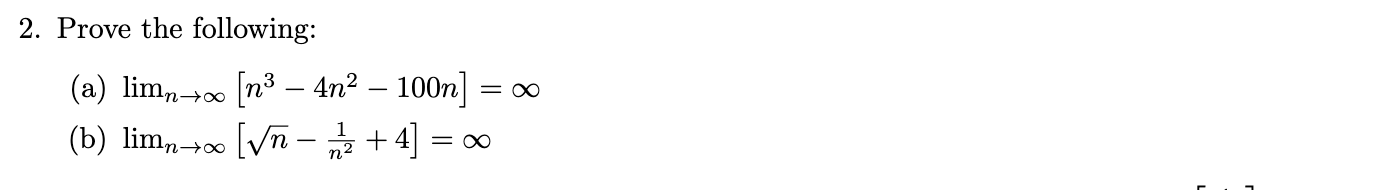
\includegraphics[width=14cm]{2.png}

\begin{proof}
  Yes, consider the scatter plot. The duplicate data has exactly the same points 
  as the original data, so the slope estimates must be the same. Furthermore, 
  consider the process of minimizng the same squared errors 
  \[\min_{\beta_0, \beta_1} \sum_{i=1}^{2n}(y_i - \beta_0 - \beta_1 x_1)^2 = \min_{\beta_0, \beta_1} 2\sum_{i=1}^n (y_i - \beta_0 - \beta_1 x_1)^2\]
  will yield exactly the same OLS estimates $\hat{\beta}_0, \hat{\beta}_1$.
\end{proof}

\includegraphics[width=14cm]{2b.png}

\begin{proof}
  
\end{proof}

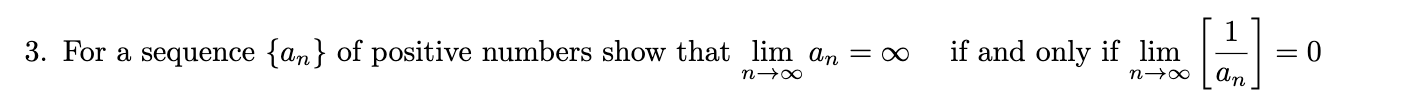
\includegraphics[width=14cm]{3.png}

\begin{proof}[Solution]

  \hfill

  \begin{enumerate}[a.]
    \item Yes; many portfolios have nonzero alpha and as betas increase, 
    decrease.
    \item Long edf1 and short edf10
  \end{enumerate}
\end{proof}

\includegraphics[width=14cm]{2_1.png}

\begin{proof}
  Note that if each $X_i$ is normal, then the sum of the $X_i$ is normal.
  \[\E(\frac{1}{N}\sum X_i) = \frac{1}{N}N\mu = \mu\]
  \[\V(\frac{1}{N}\sum X_i) = \frac{1}{N^2}\V(\sum X_i) = \frac{1}{N^2} N\sigma^2 = \frac{\sigma^2}{N}\]
  because the $X_i$ are iid and so the covariances are all $0$. Therefore, 
  \[\bar{X}_n \sim N(\mu, \frac{\sigma^2}{N})\]
\end{proof}

\includegraphics[width=14cm]{2_2.png}

\begin{proof}
  Population variance is known, and so we can use the z-statistic and not the 
  t-statistic. Our confidence is 
  \[[\bar{X}_{100} \pm \frac{4}{10} * 1.96]\]
\end{proof}

\includegraphics[width=14cm]{3_1.png}

\begin{proof}
  Note the important fact of the CAPM that despite varying risk-tolerances, all 
  investors hold the tangent portfolio, just weighted differently towards the tangent portfolio and the 
  risk free asset. Thus, we seek to show that 
  \[\rho = \dfrac{\C(w * R_m, R_m)}{\sqrt{\V(w * R_m)} \sqrt{\V(R_m)}} = 1\]
  \[= \dfrac{w \V(R_m)}{w \V(R_m)} = 1\]
  Recall the property that $\C(aX, Y) = a\C(X, Y)$ for the numerator and 
  $\V(aX) = a^2\V(X)$ in the denominator.
\end{proof}

\includegraphics[width=14cm]{3_6.png}

\begin{proof}
  Note that
  \[\hat{\beta}_1 = \dfrac{\C(X, Y)}{\sqrt{\V(X)\V(Y)}} \approx \dfrac{\sum_i (x_i - \bar{x})(y_i - \bar{y})}{\sum_j (x_j - \bar{x})^2} = \sum_i c_i y_i\]
  where 
  \[c_i := \dfrac{x_i - \bar{x}}{\sum_j (x_j - \bar{x})^2}\]
  Fixing $x_i, y_i | x_i \sim N(\beta_1x_i, \sigma^2)$ and so since $\hat{\beta}_1$ is the sum of normal distributions, 
  it is also a normal distribution.

\end{proof}

\end{document}

